\subsection{Caracterização microestrutural}

\subsubsection{Efeito da temperatura de têmpera}

\begin{frame}[t]{Caracterização microestrutural}{Diferentes temperaturas de têmpera}
	TP = 300 °C / 15 min

	\begin{figure}
		\centering
		\includegraphics[width=.9\textwidth]{../texto/img/micrografias/MEV/PT300.pdf}
	\end{figure}
\end{frame}

\subsubsection{Efeito da temperatura de partição}
%\begin{frame}[t]{Caracterização microestrutural}
	%\begin{block}{MO em baixo aumento (TT=170°C \& TP=300°C)}
		%\begin{itemize}
			%\item Regiões de contorno de célula eutética (segregadas) apresentam padrão de ataque branco: $\gamma$
			%\item Padrão se repete para todas as demais condições
		%\end{itemize}
%
		%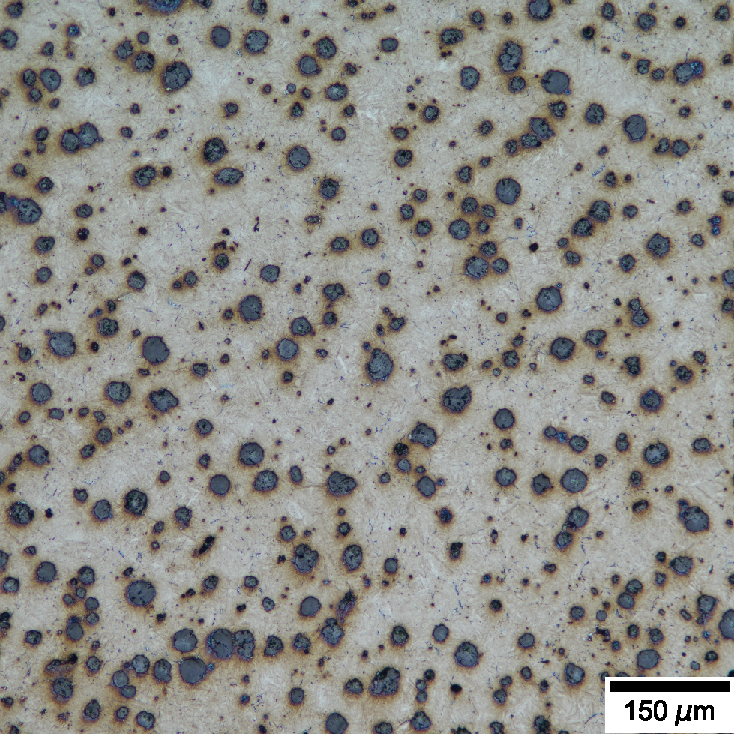
\includegraphics[height=5.5cm]{../texto/img/micrografias/MO/TT140TP300/100x-1.pdf}
	%\end{block}
%\end{frame}

%\begin{frame}[t]{Caracterização microestrutural}{Diferentes temperaturas de têmpera}
	%\begin{itemize}
		%\item Difícil reconhecimento de diferentes frações volumétricas de $\alpha\text{\textquoteright}$
		%\item No entanto, $\alpha$ bainítico possui diferentes escalas
	%\end{itemize}
%
	%\begin{figure}[c]
	%\includegraphics[width=4cm]{../texto/img/micrografias/MEV/TT140TP300/10k-3.pdf}\,
	%\includegraphics[width=4cm]{../texto/img/micrografias/MEV/TT170TP300/10k-1_semSetas.pdf}\vspace{1pt}
	%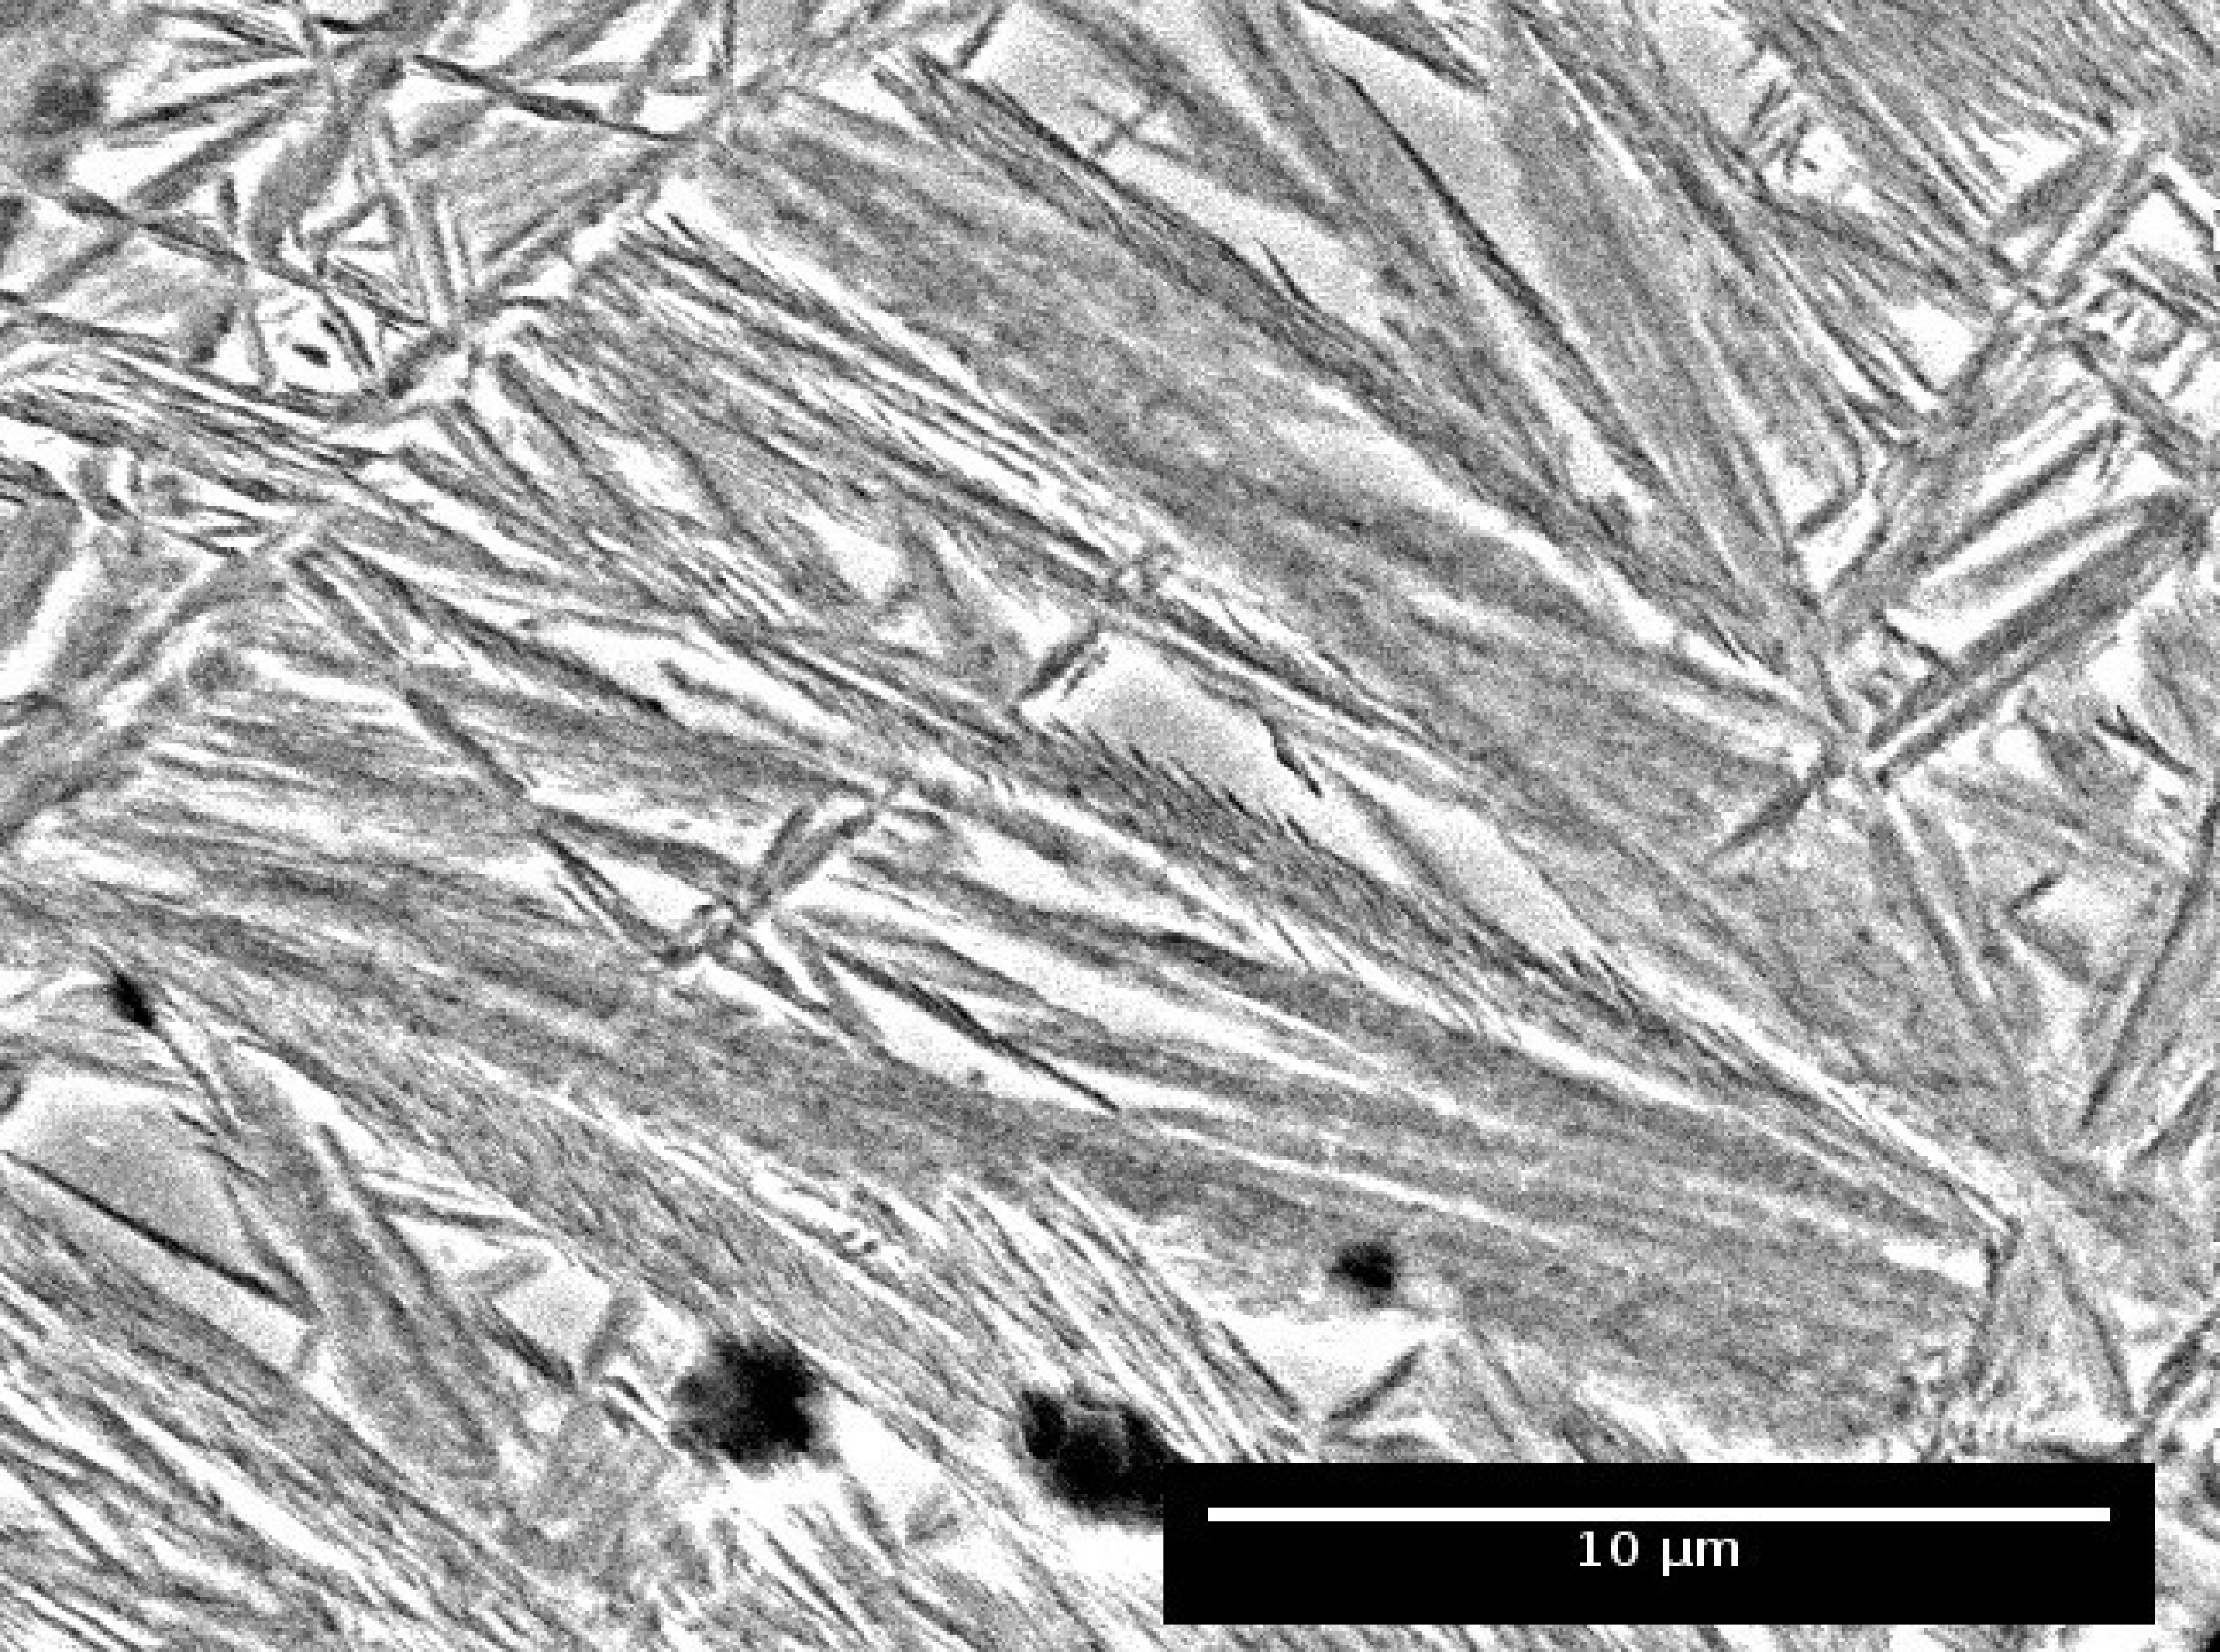
\includegraphics[width=4cm]{../texto/img/micrografias/MEV/TT200TP300/10k-1.pdf}
	%\end{figure}
%\end{frame}

%%%%%%%%%%%%%%%%%%
\begin{frame}[t]{Caracterização microestrutural}{Diferentes temperaturas de partição}
	\begin{block}{Têmpera a 170 °C e partição a 375 °C / 15 min}
	\begin{itemize}
		\item Áreas brancas / alto relevo: austenita
		\item Placas de martensita (setas azuis) e produto acicular: ferrita bainítica (setas vermelhas)
	\end{itemize}

	\begin{figure}
		\centering
		\includegraphics<1>[width=.7\textwidth]{../texto/img/micrografias/MO/TT170TP375/1000x-1.pdf}
		\includegraphics<2>[width=.65\textwidth]{../texto/img/micrografias/MEV/TT170TP375/25k-4}
	\end{figure}
	\end{block}
\end{frame}

\begin{frame}[t]{Caracterização microestrutural}{Diferentes temperaturas de partição}
	\begin{block}{Têmpera a 170 °C e partição a 300 °C / 15 min}
	\begin{itemize}
		\item Descrição semelhante, mas ferrita bainítica é mais refinada
		\item Baixo aumento: concentração de austenita em áreas de segregação
	\end{itemize}

	\begin{figure}
		\centering
		\includegraphics<1>[width=.7\textwidth]{../texto/img/micrografias/MO/TT170TP300/1000x-2.pdf}
		\includegraphics<2>[width=.65\textwidth]{../texto/img/micrografias/MEV/TT170TP300/25k-2}
		\includegraphics<3>[width=.7\textwidth]{../texto/img/micrografias/MO/TT170TP300/100x-1}
	\end{figure}
	\end{block}
\end{frame}

\begin{frame}[t]{Caracterização microestrutural}{Diferentes temperaturas de partição}
	\begin{block}{Têmpera a 170 °C e partição a 250 °C / 15 min}
	\begin{itemize}
		\item Menor fração volumétrica de ferrita bainítica
	\end{itemize}

	\begin{figure}
		\centering
		\includegraphics<1>[width=.8\textwidth]{../texto/img/micrografias/MO/TT170TP250/1000x-2.pdf}
		\includegraphics<2>[width=.7\textwidth]{../texto/img/micrografias/MEV/TT170TP250/25k-1}
		\includegraphics<3>[width=.7\textwidth]{../texto/img/micrografias/MEV/TT170TP250/50k-4}
	\end{figure}
	\end{block}
\end{frame}

\begin{frame}[t]{Caracterização microestrutural}{Diferentes temperaturas de partição}
	\begin{block}{Têmpera a 170 °C e partição a 200 °C / 15 min}
	\begin{itemize}
		\item Não são observados produtos aciculares
	\end{itemize}

	\begin{figure}
		\centering
		\includegraphics<1>[width=.7\textwidth]{../texto/img/micrografias/MEV/TT170TP200/25k-2.pdf}
	\end{figure}
	\end{block}
\end{frame}

\begin{frame}[t]{Caracterização microestrutural}{Diferentes temperaturas de partição}
	\begin{block}{Têmpera a 170 °C e partição a 200 °C / 2 h}
	\begin{itemize}
		\item Para longos tempos se observam produtos refinados em morfologia de zigue-zague
		\item Lembra martensita formada autocataliticamente (bursts)
	\end{itemize}

	\begin{figure}
		\centering
		\includegraphics<1>[width=.65\textwidth]{../texto/img/micrografias/MEV/TT170TP200-2h/10k-1.pdf}
		\includegraphics<2>[width=.65\textwidth]{../texto/img/micrografias/MEV/TT170TP200-2h/25k-1.pdf}
	\end{figure}
	\end{block}
\end{frame}

\begin{frame}[t]{Caracterização microestrutural}{Diferentes temperaturas de partição}
	\begin{block}{Têmpera a 170 °C e partição a 450 °C / 15 min}
	\begin{itemize}
		\item Ainda que DRX e dilatometria não prevejam austenita, são vistas áreas desta fase (áreas segregadas)
	\end{itemize}

	\begin{figure}
		\centering
		\includegraphics<1>[width=.7\textwidth]{../texto/img/micrografias/MO/TT170TP450/1000x-1.pdf}
		\includegraphics<2>[width=.65\textwidth]{../texto/img/micrografias/MEV/TT170TP450/10k-8.pdf}
		\includegraphics<3>[width=.65\textwidth]{../texto/img/micrografias/MEV/TT170TP450/25k-1.pdf}
	\end{figure}
	\end{block}
\end{frame}

\begin{frame}[t]{Caracterização microestrutural}{Diferentes temperaturas de partição}
	\begin{block}{Têmpera a 170 °C e partição a 450 °C / 2h}
	\begin{itemize}
		\item Dispersão muito fina de carbonetos é vista (principalmente para tempos longos)
	\end{itemize}

	\begin{figure}
		\centering
		\includegraphics<1>[width=.65\textwidth]{../texto/img/micrografias/MEV/TT170TP450-2h/10k-1.pdf}
		\includegraphics<2>[width=.65\textwidth]{../texto/img/micrografias/MEV/TT170TP450-2h/50k-1.pdf}
	\end{figure}
	\end{block}
\end{frame}
